\chapter{Izdvojeni detalji implementacije} \label{chapter:implementation}
Detalji izdvojeni u ovom poglavlju ključni su za razumijevanje sigurnosnog modela aplikacije, sa tog aspekta posebno su zanimljiva dva objekta, \texttt{Attendance} i \texttt{Session}, koji u osnovi predstavljaju proširene kriptografski potpisane SPIM i SESS objekte.

\section{Podatkovni i kriptografski primitivi}
\subsection{SPIM paket}
Spim u širem smislu predstavlja vremensko-lokacijski objekat (\textit{en. SPace-tIMe}), koji korištenjem kriptografske obrade poprima karakteristike lokacijskog dokaza. Polazna struktura za formiranje SPIM objekta sastoji se iz korisničkog imena studenta, geografske širine, geografske dužine i trenutnog vremena na studentovom mobilnom uređaju. Ovako komponovan objekat predstavlja implementaciju lokacijskog dokaza u užem smislu i koristi se dalje kao osnovni podatkovni primitiv za dalju kriptografsku obradu. Cjelovit prikaz JSON oblika kriptografski obrađenog SPIM objekta dat je u listingu \ref{code:json_spime}.

\begin{code}
    \inputminted{text}{material/logit_tag.txt}
    \captionof{listing}{JSON reprezentacija SPIM objekta}
    \label{code:json_spime}
\end{code}

\paragraph*{}
Navedene vrijednosti stringova korisničkog imena studenta, geografske širine, geografske dužine i trenutnog vremena se lančaju u jedan string izloženim redoslijedom i takav string se potpisuje korištenjem RSA kriptografije, tako potpisan paket u obliku JSON objekta (prikazan u listingu iznad) šalje se na profesorski master uređaj, gdje se dodaju podaci sesije, u vidu jedinstvenog identifikatora sesije (SID), te se potpisano studentsko prisustvo obilježava jedinstvenim heksadecimalnim identifikatorom AID izvedenim iz potpisa prisustva putem SHA256 hash funkcije, navedene vrijednosti, SID i AID se lančaju u jedan binarni string i potpisuju od strane profesora (CONFSIG), naknadno se na osnovu SHA256 hash vrijednosti CONFSIG profesorskog potpisa formira finalni identifikator potvrde prisustva CID, time se završava kriptografsko osiguravanje valjanosti prisustva u smislu SPIM objekta, u cilju bolje preglednosti slika \ref{fig:dia_class} prikazuje dijagram klasa navedenih objekata sa anotacijom navedenom ispod.

\begin{figure}[H]
    \centering
    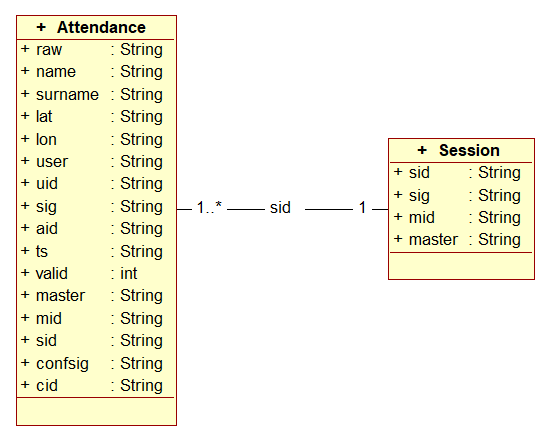
\includegraphics[width=0.6\textwidth]{material/classmodel}
    \caption{Dijagram klasa SPIM i SESS objekata}
    \label{fig:dia_class}
\end{figure}
\begin{description}[align=right,labelwidth=2cm,noitemsep]
    \item [raw] serijalizirana string JSON verzija objekta
    \item [name] ime studenta
    \item [surname] prezime studenta
    \item [lat] geografska širina student
    \item [lon] geografska dužina student
    \item [user] ZAMGER korisničko ime studenta
    \item [uid] User ID - SHA2 hex hash javnog ključa studenta
    \item [sig] hex potpis SPIM-a (user:lat:lot:ts)
    \item [aid] Attendance ID - hex SHA2 hash \texttt{sig} potpisa
    \item [ts] vrijeme na studentovom uređaju
    \item [valid] validation cache
    \item [master] ZAMGER korisničko ime profesora
    \item [mid] Master ID - SHA2 hex hash javnog ključa profesora
    \item [sid] Session ID - identifikator profesorove sesije
    \item [confsig] Master Conf. profesorov hex potpis (sid:aid)
    \item [cid] Confirmation ID - SHA2 hex hash confsig-a
\end{description}

\paragraph*{}
Fizički predstavljen opisani SPIM objekat manji je od 1 KB te je pored brzog NFC isl. elektronskog transfera moguće izvršiti prenos alternativnim metodama, kao posebno pogodna čini se QR kod reprezentacija\cite{soon2008qr} i prenos, koja može biti vrlo korisna u slučaju da nijedan od uređaja ne posjeduje NFC modem. Navedeni modus nije implementiran u aplikaciji i dat je kao sugestija zaobilaženja hardverskih ograničenja, primjer QR oblika ranije datog SPIM objekta prikazan je na slici \ref{img:qr}.

\paragraph*{}
Dati QR prikaz je čitljiv ali je uočljiva visoka gustina zapisa koja može predstavljati problem u slučaju lošije kvalitete medija prikaza, u tom slučaju, kompletan SPIM paket moguće je značajno smanjiti zamjenom korištenog RSA kriptosistema za kriptosistem baziran na eliptičnim krivim, budući da su ključevi korišteni u tom slučajnu znatno kraći\cite{atmelecc}, dužina navedenog potpisa bila bi smanjena sa 512 na minimalno 71 bajt\cite{cheneau2009ecc} navedeni pristup nije prihvaćen u okviru ovog rada zbog povećanja kompleksnosti pokaznog sistema, no praktična implementacija moguća je bez većih programskih izmjena.

\begin{figure}[H]
    \centering
    \begin{subfigure}{.5\textwidth}
        \centering
        
\includegraphics[width=.8\textwidth]{material/logit_qr}
        \caption{oblik korištenjem RSA potpisa}
        \label{img:qr_rsa}
    \end{subfigure}%
    \begin{subfigure}{.5\textwidth}
        \centering
        
\includegraphics[width=.8\textwidth]{material/logit_qr_ec}
        \caption{oblik korištenjem ECC potpisa}
        \label{img:qr_ecc}
    \end{subfigure}
    \caption{QR oblik SPIM objekta}%
    \label{img:qr}
\end{figure}

\subsection{SESS paket}
Dodatno se za SESS objekat prilikom finaliziranja sesije na LAPI serveru vrši prikupljanje svih CID potpisa koji pripadaju datoj sesiji, te se CID vrijednosti ulančane hronološkim redoslijedom potpisuju LAPI ključem koji se nalazi samo na LAPI hardverskom uređaju, stoga je sigurnost LAPI servera od ključne važnosti za sigurnost ukupnog sistema. Ovako potvrđena sesija ne može biti naknadno mijenjana, lažirana ili porečena izvan LAPI izvršnog okruženja.

\cleardoublepage
\section{Pregled implementacije}
\subsection{MainActivity}
Nakon prvobitnog pokretanja aplikacije a za daljnje uspješno korištenje neophodno je izvršiti autentifikaciju korisnika putem nekog već postojećeg korisničkog repozitorija, te generisati pripadajući virtualizirani sigurni element. Navedene aktivnosti izvršavaju se unutar \texttt{MainActivity} glavnog početnog prozora Logit aplikacije, prikaz relevantnog dijela koda za generisanje virtualiziranog sigurnog elementa dat je u listingu \ref{code:main_activity_keygen} ispod.

\begin{code}
\begin{minted}{python}
KeyPairGenerator kpg = KeyPairGenerator.getInstance(
        "RSA", "AndroidKeyStore");
Calendar start = Calendar.getInstance();
Calendar end = Calendar.getInstance();
end.add(Calendar.YEAR, 1);

KeyPairGeneratorSpec spec =
        new KeyPairGeneratorSpec.Builder(this).setAlias("etf_logit_" + ts)
                .setKeySize(2048)
                .setSubject(new X500Principal("CN=users.etf.ba"))
                .setSerialNumber(BigInteger.valueOf(tsLong))
                .setStartDate(start.getTime()).setEndDate(end.getTime()).build();

kpg.initialize(spec);

KeyPair kp = kpg.generateKeyPair();

KeyStore ks = KeyStore.getInstance("AndroidKeyStore");
ks.load(null);
\end{minted}
\captionof{listing}{MainActivity - generisanje RSA para ključeva}
\label{code:main_activity_keygen}
\end{code}

\paragraph*{}
Sigurnosni element generisan kao u primjeru iznad dalje se pohranjuje na korisničkom uređaju, gdje privatni dio nikada ne napušta uređaj i dostupan je isključivo Logit aplikaciji putem Android KeyStore providera. Javni dio se koristi kao dio identifikatora korisnika, te se dodatno pohranjuje i na Logit API korisnički repozitorij za potrebe identifikacije i verifikacije potpisa lokacijskog paketa.

\subsection{LogitAPDUService}
Ekstenzija Androidovog native interfejsa \texttt{HostApduService} koji za instaliranu aplikaciju sa \texttt{android.permission.BIND\_NFC\_SERVICE} permisijom vrši pokretanje HCE emulatora prilikom svakog starta operativnog sistema, emulator se u ovom slučaju ponaša kao generički NFC NTAG sa korisnički programiranom memorijom u obliku NDEF poruke koja prenosi jedinstveni potpisan studentski lokacijski dokaz. Navedena servisna komponenta aplikacije aktivna je svaki put dok je i ekran uređaja aktivan ili dok korisnik sam ne zaustavi pripadajući servis. Navedene funkcionalnosti postižu se uključivanjem dijela koda datog u nastavku unutar \texttt{<application>} direktive manifest fajla kao što je navedeno u listingu \ref{code:manifest}.

\begin{code}
\begin{minted}{python}
<service
    android:name=".LogitApduService"
    android:permission="android.permission.BIND_NFC_SERVICE">
    <intent-filter>
        <action android:name="android.nfc.cardemulation.action.HOST_APDU_SERVICE" />

        <category android:name="android.intent.category.DEFAULT" />
    </intent-filter>

    <meta-data
        android:name="android.nfc.cardemulation.host_apdu_service"
        android:resource="@xml/apduservice" />
</service>
\end{minted}
\captionof{listing}{LogitApduService deklaracija unutar Android manifesta}
\label{code:manifest}
\end{code}

\paragraph*{}
Nadalje \texttt{LogitAPDUService} sadrži logiku za ispravno konstruisanje i formatiranje NDEF paketa\cite{tindef} lokacijskog dokaza i njegovo potpisivanje, te ostalu neophodnu kriptografsku obradu. U nastavku će biti dat prikaz kompletnog servisa sa komentarima relevantnih dijelova.

\paragraph*{}
Kod dat u okviru listinga \ref{code:service_const} deklariše konstantne vrijednosti brojnih dijelova neophodnih za kontrukciju standardne NDEF poruke, između ostalog \textit{capability} fajl koji predstavlja svojevrsno zaglavlje prije NDEF paketa.

\begin{code}
\begin{minted}{python}
final static int APDU_INS = 1;
final static int APDU_P1 = 2;
final static int APDU_P2 = 3;
final static int APDU_SELECT_LC = 4;
final static int APDU_READ_LE = 4;
final static int FILEID_CC = 0xe103;
final static int FILEID_NDEF = 0xe104;
final static byte INS_SELECT = (byte) 0xa4;
final static byte INS_READ = (byte) 0xb0;
final static byte INS_UPDATE = (byte) 0xd6;
final static byte P1_SELECT_BY_NAME = (byte) 0x04;
final static byte P1_SELECT_BY_ID = (byte) 0x00;
final static int DATA_OFFSET = 5;

final static byte[] DATA_SELECT_NDEF = {
        (byte) 0xd2, (byte) 0x76, (byte) 0x00, (byte) 0x00,
        (byte) 0x85, (byte) 0x01, (byte) 0x01
    };
final static byte[] RET_COMPLETE = {(byte) 0x90, (byte) 0x00};
final static byte[] RET_NONDEF = {(byte) 0x6a, (byte) 0x82};
final static byte[] FILE_CC = {
        (byte) 0x00, (byte) 0x0f,       // CCLEN - CC container size
        (byte) 0x20,                    // Mapping version
        (byte) 0x04, (byte) 0xff,       // MLe - max. read size
        (byte) 0x08, (byte) 0xff,       // MLc - max. update size

        // TLV Block (NDEF File Control)
        (byte) 0x04,                    // Tag - Block type
        (byte) 0x06,                    // Length
        (byte) 0xe1, (byte) 0x04,       // File identifier
        (byte) 0x04, (byte) 0xff,       // Max. NDEF file size
        (byte) 0x00,                    // R permission
        (byte) 0x00,                    // W permission
    };
\end{minted}
\captionof{listing}{LogitAPDUService - konstante za emulaciju taga i NDEF poruke}
\label{code:service_const}
\end{code}

\paragraph*{}
Metoda generateSignature instancira lokacijske servise i vrši konstukciju paketa lokacijskog dokaza kao i kriptografskih primitiva neophodnih za potpisivanje istog. Za konstrukciju lokacijskog dokaza neophodno je pribaviti trenutno vrijeme uređaja, kao u listingu \ref{code:service_datetime}.

\begin{code}
\begin{minted}{python}
Long tsLong = System.currentTimeMillis() / 1000;
String ts = tsLong.toString();
byte[] signature;
\end{minted}
\captionof{listing}{LogitAPDUService - dobavljanje trenutnog vremena uređaja}
\label{code:service_datetime}
\end{code}

\paragraph*{}
Nakon toga kodom navedenim u listingu \ref{code:service_keystore} vrši se instanciranje i učitavanja Android KeyStore objekta koji sadrži korisnički par ključeva neophodnih za potpisivanje lokacijskog paketa.

\begin{code}
\begin{minted}{python}
KeyStore ks = KeyStore.getInstance("AndroidKeyStore");
ks.load(null);
KeyStore.ProtectionParameter pp = new KeyStore.PasswordProtection(null);
\end{minted}
\captionof{listing}{LogitAPDUService - instanciranje KeyStore objekta}
\label{code:service_keystore}
\end{code}

\paragraph*{}
Nadalje kod prikazan u listingu \ref{code:service_keyload} iz \texttt{KeyStore} objekta učitava najažurniji par ključeva na korisničkom uređaju u cilju emulacije sigurnog elementa.

\begin{code}
\begin{minted}{python}
Enumeration<String> aliases = ks.aliases();
String alias = aliases.nextElement();
Entry entry = ks.getEntry(alias, pp);
\end{minted}
\captionof{listing}{LogitAPDUService - učitavanje važećeg para ključeva}
\label{code:service_keyload}
\end{code}

\paragraph*{}
Zbog potrebe za što kompaktnijim prenosom podataka za sve vrijednosti gdje je to moguće generišu se hash preslikavanja koja se kasnije koriste za verifikaciju i pohranjivanje. Za potrebe generisanja hash vrijednosti instancira se SHA-256 \texttt{MessageDigest} objekat kako je prikazano u listingu \ref{code:service_hash} ispod.

\begin{code}
\begin{minted}{python}
MessageDigest md = MessageDigest.getInstance("SHA-256");
\end{minted}
\captionof{listing}{LogitAPDUService - instanciranje MessageDigest hash generatora}
\label{code:service_hash}
\end{code}

\paragraph*{}
Iz virtualiziranog sigurnog elementa dalje učitavamo korisnički certifikat sa javnim ključem, te za potrebe verifikacije identiteta heksadecimalnu reprezentaciju njegove hash vrijednosti pripremamo za uključenje u paket lokacijskog dokaza, prikazano listingom \ref{code:service_cert}.

\begin{code}
\begin{minted}{python}
Certificate c = ks.getCertificate(alias);
byte [] pubKey = c.getPublicKey().getEncoded();
md.update(pubKey, 0, pubKey.length);
byte [] pubKeyHash = md.digest();
String pubKeyHashString = LogitApplication.toHext(pubKeyHash);
\end{minted}
\captionof{listing}{LogitAPDUService - učitavanje korisničkog certifikata}
\label{code:service_cert}
\end{code}

\paragraph*{}
Zatim iz virtualiziranog sigurnog elementa, kao u listingu \ref{code:service_privkey} - korištenjem korisničkog privatnog ključa pripremamo objekat koji vrši potpisivanje lokacijskog paketa.

\begin{code}
\begin{minted}{python}
Signature s = Signature.getInstance("SHA256withRSA");
s.initSign(((PrivateKeyEntry) entry).getPrivateKey());
SharedPreferences userData = getSharedPreferences("UserData", 0);
\end{minted}
\captionof{listing}{LogitAPDUService - učitavanje privatnog ključa}
\label{code:service_privkey}
\end{code}

\paragraph*{}
Dio lokacijskog paketa koji je pokriven korisničkim digitalnim potpisom sadrži korisničko ime, lokacijske parametre geografske dužine i širine, te vrijeme uređaja u trenutku kreiranja digitalnog potpisa. Lokacijski paket se generiše na način prikazan u listingu \ref{code:service_package}.

\begin{code}
\begin{minted}{python}
String sigPkg = userData.getString("user", "unknown") +
        ":" + location.getLatitude() +
        ":" + location.getLongitude() +
        ":" + ts;
\end{minted}
\captionof{listing}{LogitAPDUService - definisanje lokacijskog paketa}
\label{code:service_package}
\end{code}

\paragraph*{}
Takav paket se na način prikazan u listingu \ref{code:service_sign} potpisuje i bilježi se njegova SHA-256 preslikana vrijednost za potrebe kasnije verifikacije.

\begin{code}
\begin{minted}{python}
s.update(sigPkg.getBytes("UTF-8"));
signature = s.sign();
\end{minted}
\captionof{listing}{LogitAPDUService - potpisivanje lokacijskog paketa}
\label{code:service_sign}
\end{code}

\paragraph*{}
Osnovni potpisani lokacijski paket se proširuje vrijednostima generisanih SHA-256 preslikavanja i osnovnim korisničkim podacima, te se prosljeđuje metodi createMessage koja formira standardizovan NDEF paket kao u listingu \ref{code:service_ndef}, takav spreman NDEF paket stavlja se na raspolaganje komponenti za prenos putem NFC protokola.

\begin{code}
\begin{minted}{python}
msg = "{\"lat\":\"" + location.getLatitude() +
        "\", \"lon\":\"" + location.getLongitude() +
        "\", \"ts\":\"" + ts +
        "\", \"sig\":\"" + LogitApplication.toHext(signature) +
        "\", \"uid\":\"" + pubKeyHashString +
        "\", \"name\":\"" + LogitApplication.toHext(userData.getString("name", "unknown").getBytes("UTF-8")) +
        "\", \"surname\":\"" + LogitApplication.toHext(userData.getString("surname", "unknown").getBytes("UTF-8")) +
        "\", \"user\":\"" + userData.getString("user", "unknown") + "\"}";

NdefMessage ndef = createMessage(msg.getBytes("UTF-8"));
byte[] ndefarray = ndef.toByteArray();

mNdefFile = new byte[ndefarray.length + 2];

mNdefFile[0] = (byte) ((ndefarray.length & 0xff00) >> 8);
mNdefFile[1] = (byte) (ndefarray.length & 0x00ff);

System.arraycopy(ndefarray, 0, mNdefFile, 2, ndefarray.length);

logitApp.setMessage(mNdefFile);
\end{minted}
\captionof{listing}{LogitAPDUService - priprema NDEF poruke za slanje}
\label{code:service_ndef}
\end{code}

\subsection{processCommandApdu}
Budući da se u prikazanom slučaju vrši emulacija pasivnog NTAG uređaja, APDU servis se izvršava u slave modu i zaprima instukcije od strane master uređaja, neophodno je implementirati parser petlju i logiku za komunikaciju sa master uređajem, unutar koje se vrši prepoznavanje zadatih instrukcija i priprema adekvatan odgovor, navedena logika implementirana je unutar \texttt{processCommandApdu} metode. Kompletna logika emulacije tag uređaja svodi se na prosljeđivanje adekvatnog zaglavlja taga i READ FROM TO binarnog protokola za čitanje memorije koju šalje master, stoga glavninu navedene metode čini jedna switch petlja koja u skladu sa zadatom komandom vraća zaglavlje ili raspon bita emuliranog taga, u ovom slučaju sadržaj koji se emulira je prošireni lokacijski paket iznad. Detalje opisane metode možete pogledati u prilogu koda u dodatku.

\subsection{AttendanceActivity}
Za ostvarivanje pune funkcionalnosti aplikacije neophodna je bila implementacija master moda za prikupljanje i obradu NDEF paketa, u ovom slučaju korisničkih potpisa, enkapsuliranih u obliku potpisanog lokacijskog paketa. \texttt{AttendanceActivity} vrši navedenu funkcionalnost te dodatno vrši provjeru valjanosti potpisa i podataka korisničkih lokacijskih paketa, u skladu sa kodom navedenim u listingu \ref{code:aa_validation}. Verifikacija korisničkih lokacijskih paketa vrši se tako što se korisnički slave podaci o vremenu i lokaciji porede sa podacima o vremenu i lokaciji master uređaja, time se osigurava zaštita od napada lažiranja podataka, te bi za takvu vrstu prevare bila neophodna koluzija dva aktera suprostavljenih interesa, što znatno umanjuje vjerovatnoću takvih napada. Moguće je podesiti vrijednosti dozvoljenih odstupanja verifikacijskih parametara izmjenom koda za tu namjenu datog u nastavku.

\begin{code}
\begin{minted}{python}
final long timediff = System.currentTimeMillis() / 1000 - Long.parseLong(tmpAttn.getTs());
final Location userLocation = new Location("MOCK");
userLocation.setLatitude(Double.valueOf(tmpAttn.getLat()));
userLocation.setLongitude(Double.valueOf(tmpAttn.getLon()));
if (Build.VERSION.SDK_INT >= 23
        && ContextCompat.checkSelfPermission(that, android.Manifest.permission.ACCESS_FINE_LOCATION ) == PackageManager.PERMISSION_GRANTED
        && ContextCompat.checkSelfPermission(that, android.Manifest.permission.ACCESS_COARSE_LOCATION) == PackageManager.PERMISSION_GRANTED
        || Build.VERSION.SDK_INT < 23) {
    FusedLocationProviderClient mFusedLocatiionClient = LocationServices.getFusedLocationProviderClient(that);
    mFusedLocatiionClient.getLastLocation().addOnSuccessListener(new OnSuccessListener<Location>() {
        @Override
        public void onSuccess(Location location) {
            Float locdiff = userLocation.distanceTo(location);
            if (Math.abs(timediff) < 300) {
                if (locdiff < 100) {
                    // Lokacija i vrijeme SLAVE uređaja su VALIDNI
                } else {
                    Toast.makeText(that, "Greška: lokacije udaljene " + locdiff.intValue() + " metara.", Toast.LENGTH_LONG).show();
                }
            } else {
                Toast.makeText(that, "Greška: vrijeme nije tačno ili je TAG zastario.", Toast.LENGTH_LONG).show();
            }
\end{minted}
\captionof{listing}{AttendanceActivity - provjera validacijskih kriterija VK1 i VK2}
\label{code:aa_validation}
\end{code}

\paragraph*{}
Da bi se izbjegla obaveza reimplementiranja NDEF protokola za podatke primljene putem NFC podatkovnog interfejsa Android nudi predefinisani intent filter za direktnu manipulaciju NDEF poruka, te je za njegovo korištenje potrebno dodati kod prikazan u listingu \ref{code:manifest_ndef} u manifest fajl Android aplikacije.

\begin{code}
\begin{minted}{python}
<intent-filter>
<action android:name="android.nfc.action.NDEF_DISCOVERED" />
<category android:name="android.intent.category.DEFAULT" />
<data android:mimeType="application/octet-stream" />
</intent-filter>
\end{minted}
\captionof{listing}{manifest - sistemska NDEF podrška za prijem poruka}
\label{code:manifest_ndef}
\end{code}

\paragraph*{}
Ostatak koda unutar \texttt{AttendanceActivity} klase koristi se za prikaz i obradu elemenata korisničkog interfejsa master moda za prikupljanje korisničkih potpisa.

\section{Korisnički interfejs}
Zbog potpunosti dokumentacijskog prikaza na slici \ref{fig:ui} data je finalna implementacija korisničkog interfejsa Logit aplikacije, oznake i numeracije rozom bojom nisu dio implementacije i poslužiti će za pojašnjenje sastavnih dijelova interfejsa i pripadajuće funkcionalnosti.

\paragraph*{}
Prikaz \ref{img:ui_l} daje uobičajenu formu za prijavu na sistem, ova forma prikazuje se samo prilikom prvog pokretanja aplikacije. Nakon prijave svakim narednim pokretanjem aplikacije aktivira se sesija za prikupljanje potpisa kao na slici \ref{img:ui_r}, zaglavlje sadrži osnovne podatke trenutno prijavljenog korisnika.

\begin{figure}[H]
    \centering
    \begin{subfigure}{.5\textwidth}
        \centering
        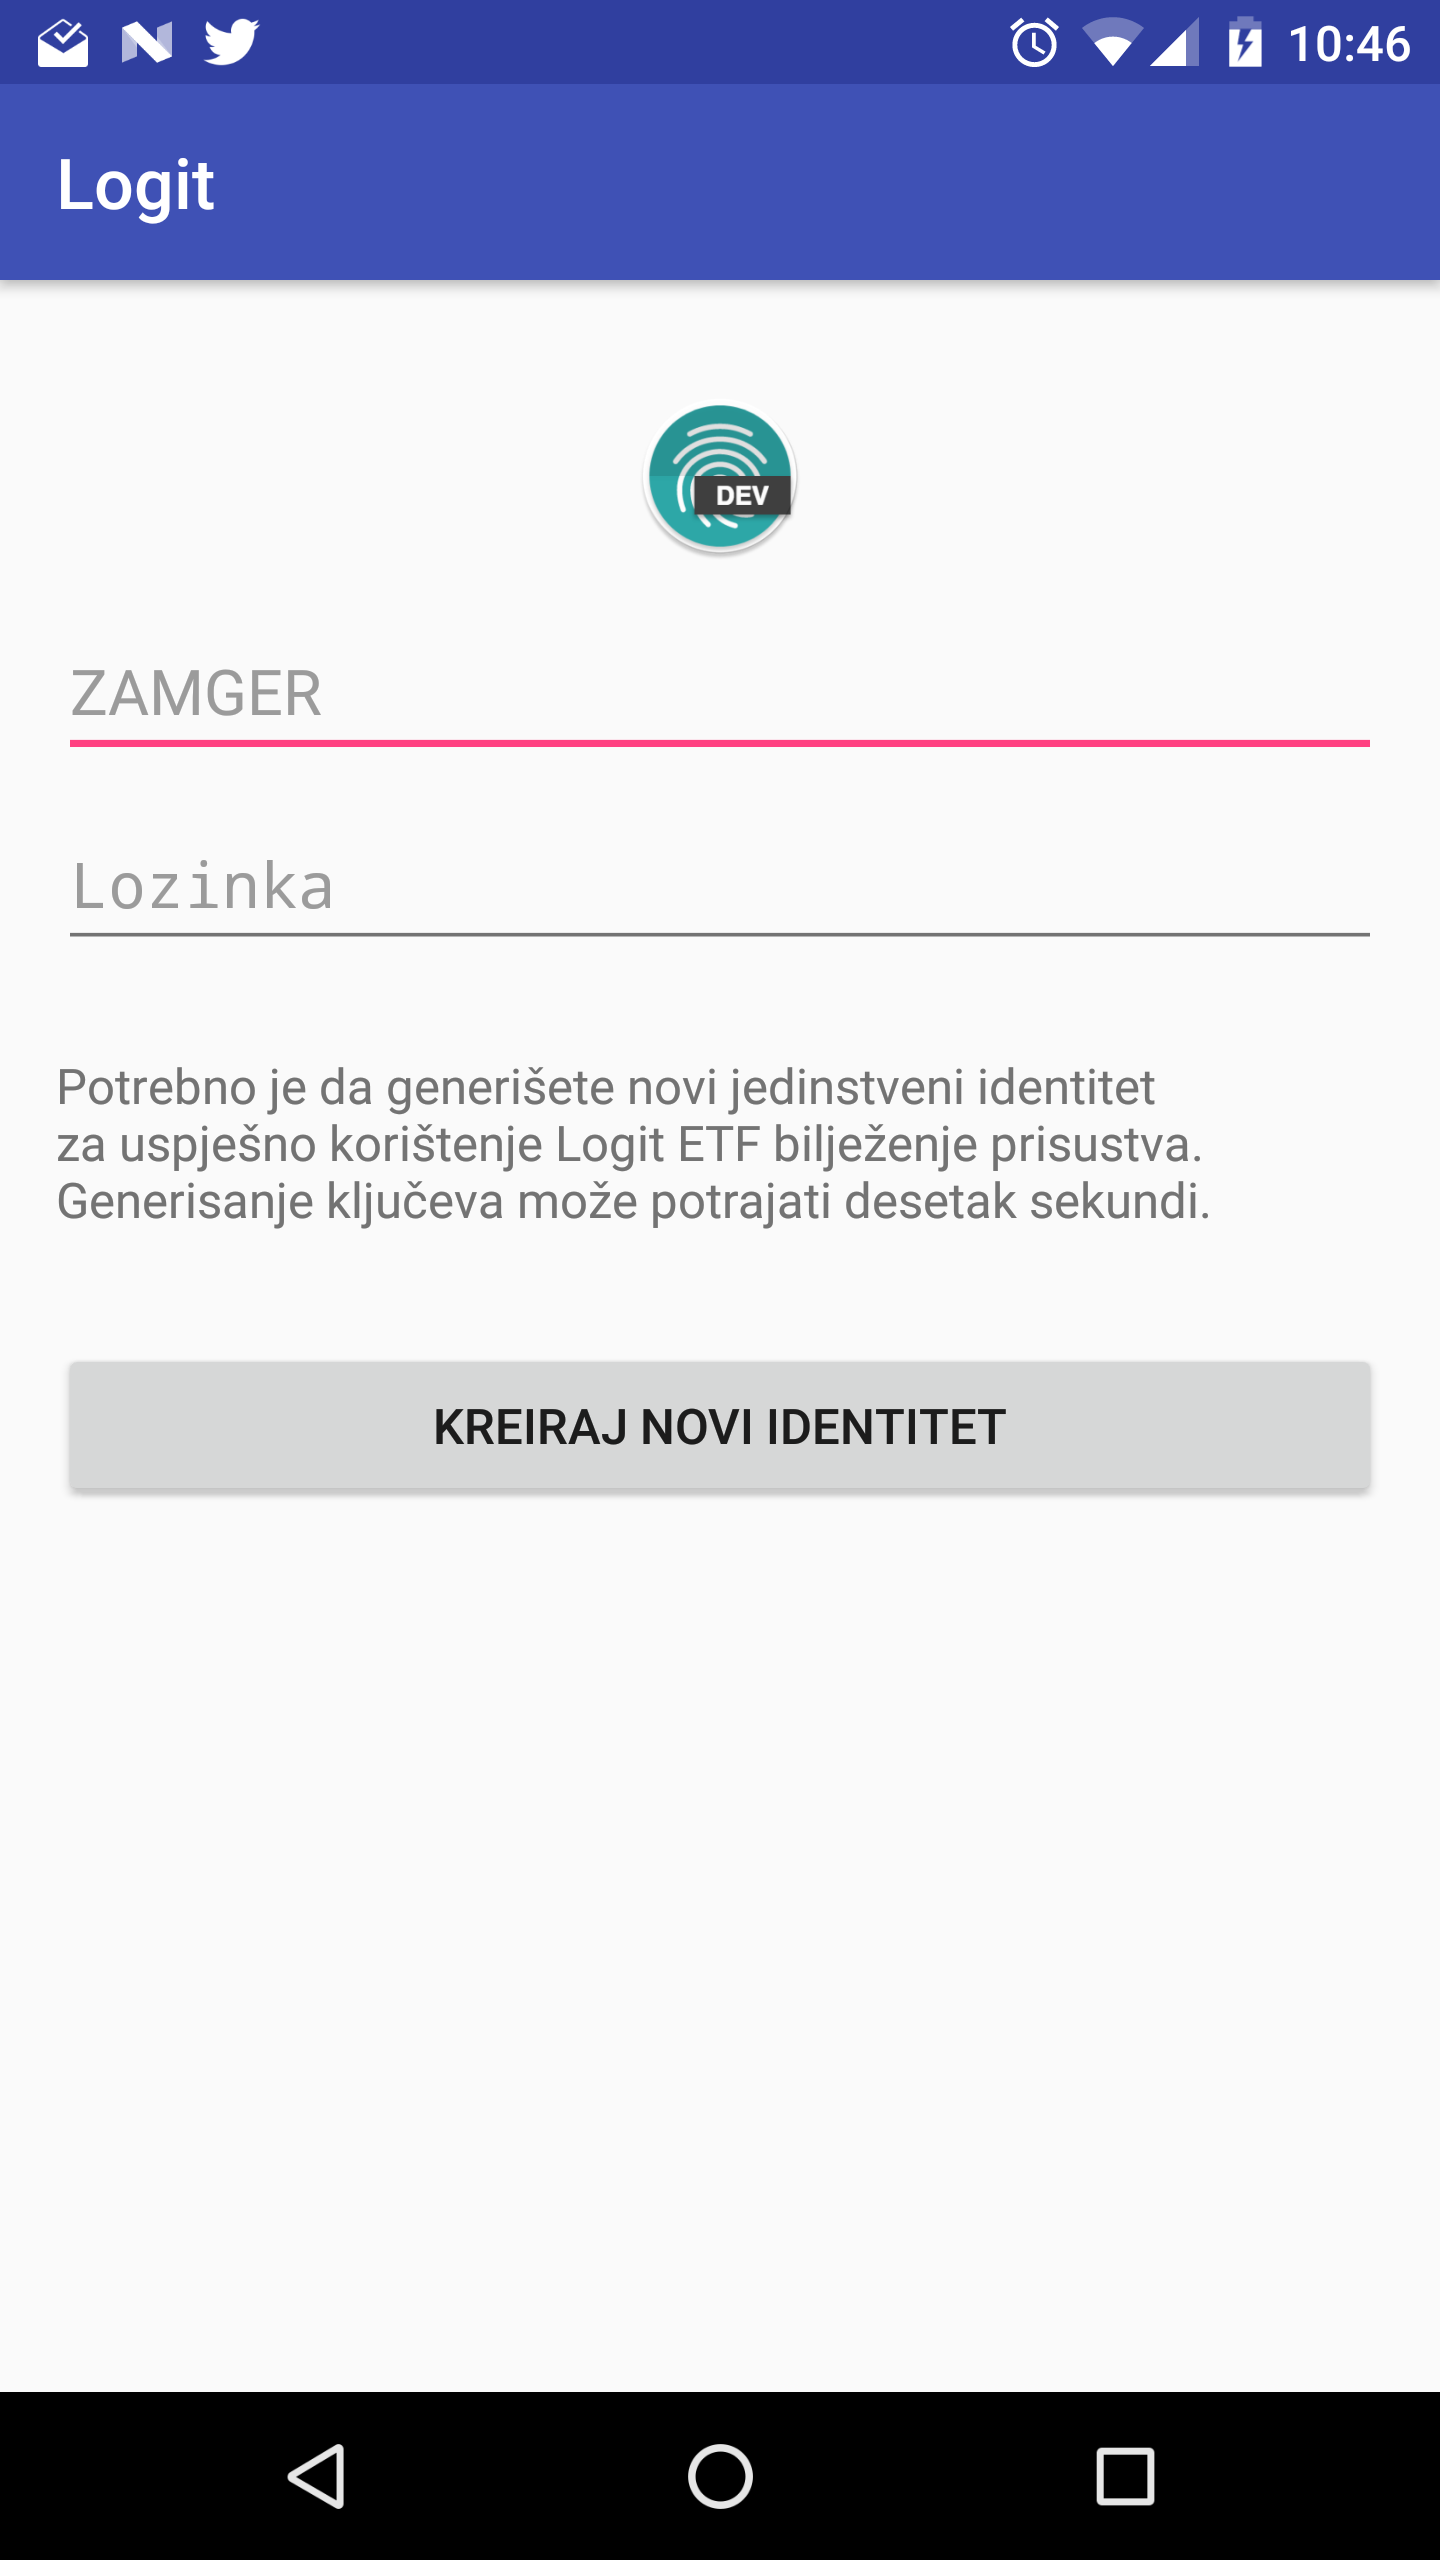
\includegraphics[width=0.9\textwidth]{material/00-login}
        \caption{forma prijave na sistem}
        \label{img:ui_l}
    \end{subfigure}%
    \begin{subfigure}{.5\textwidth}
        \centering
        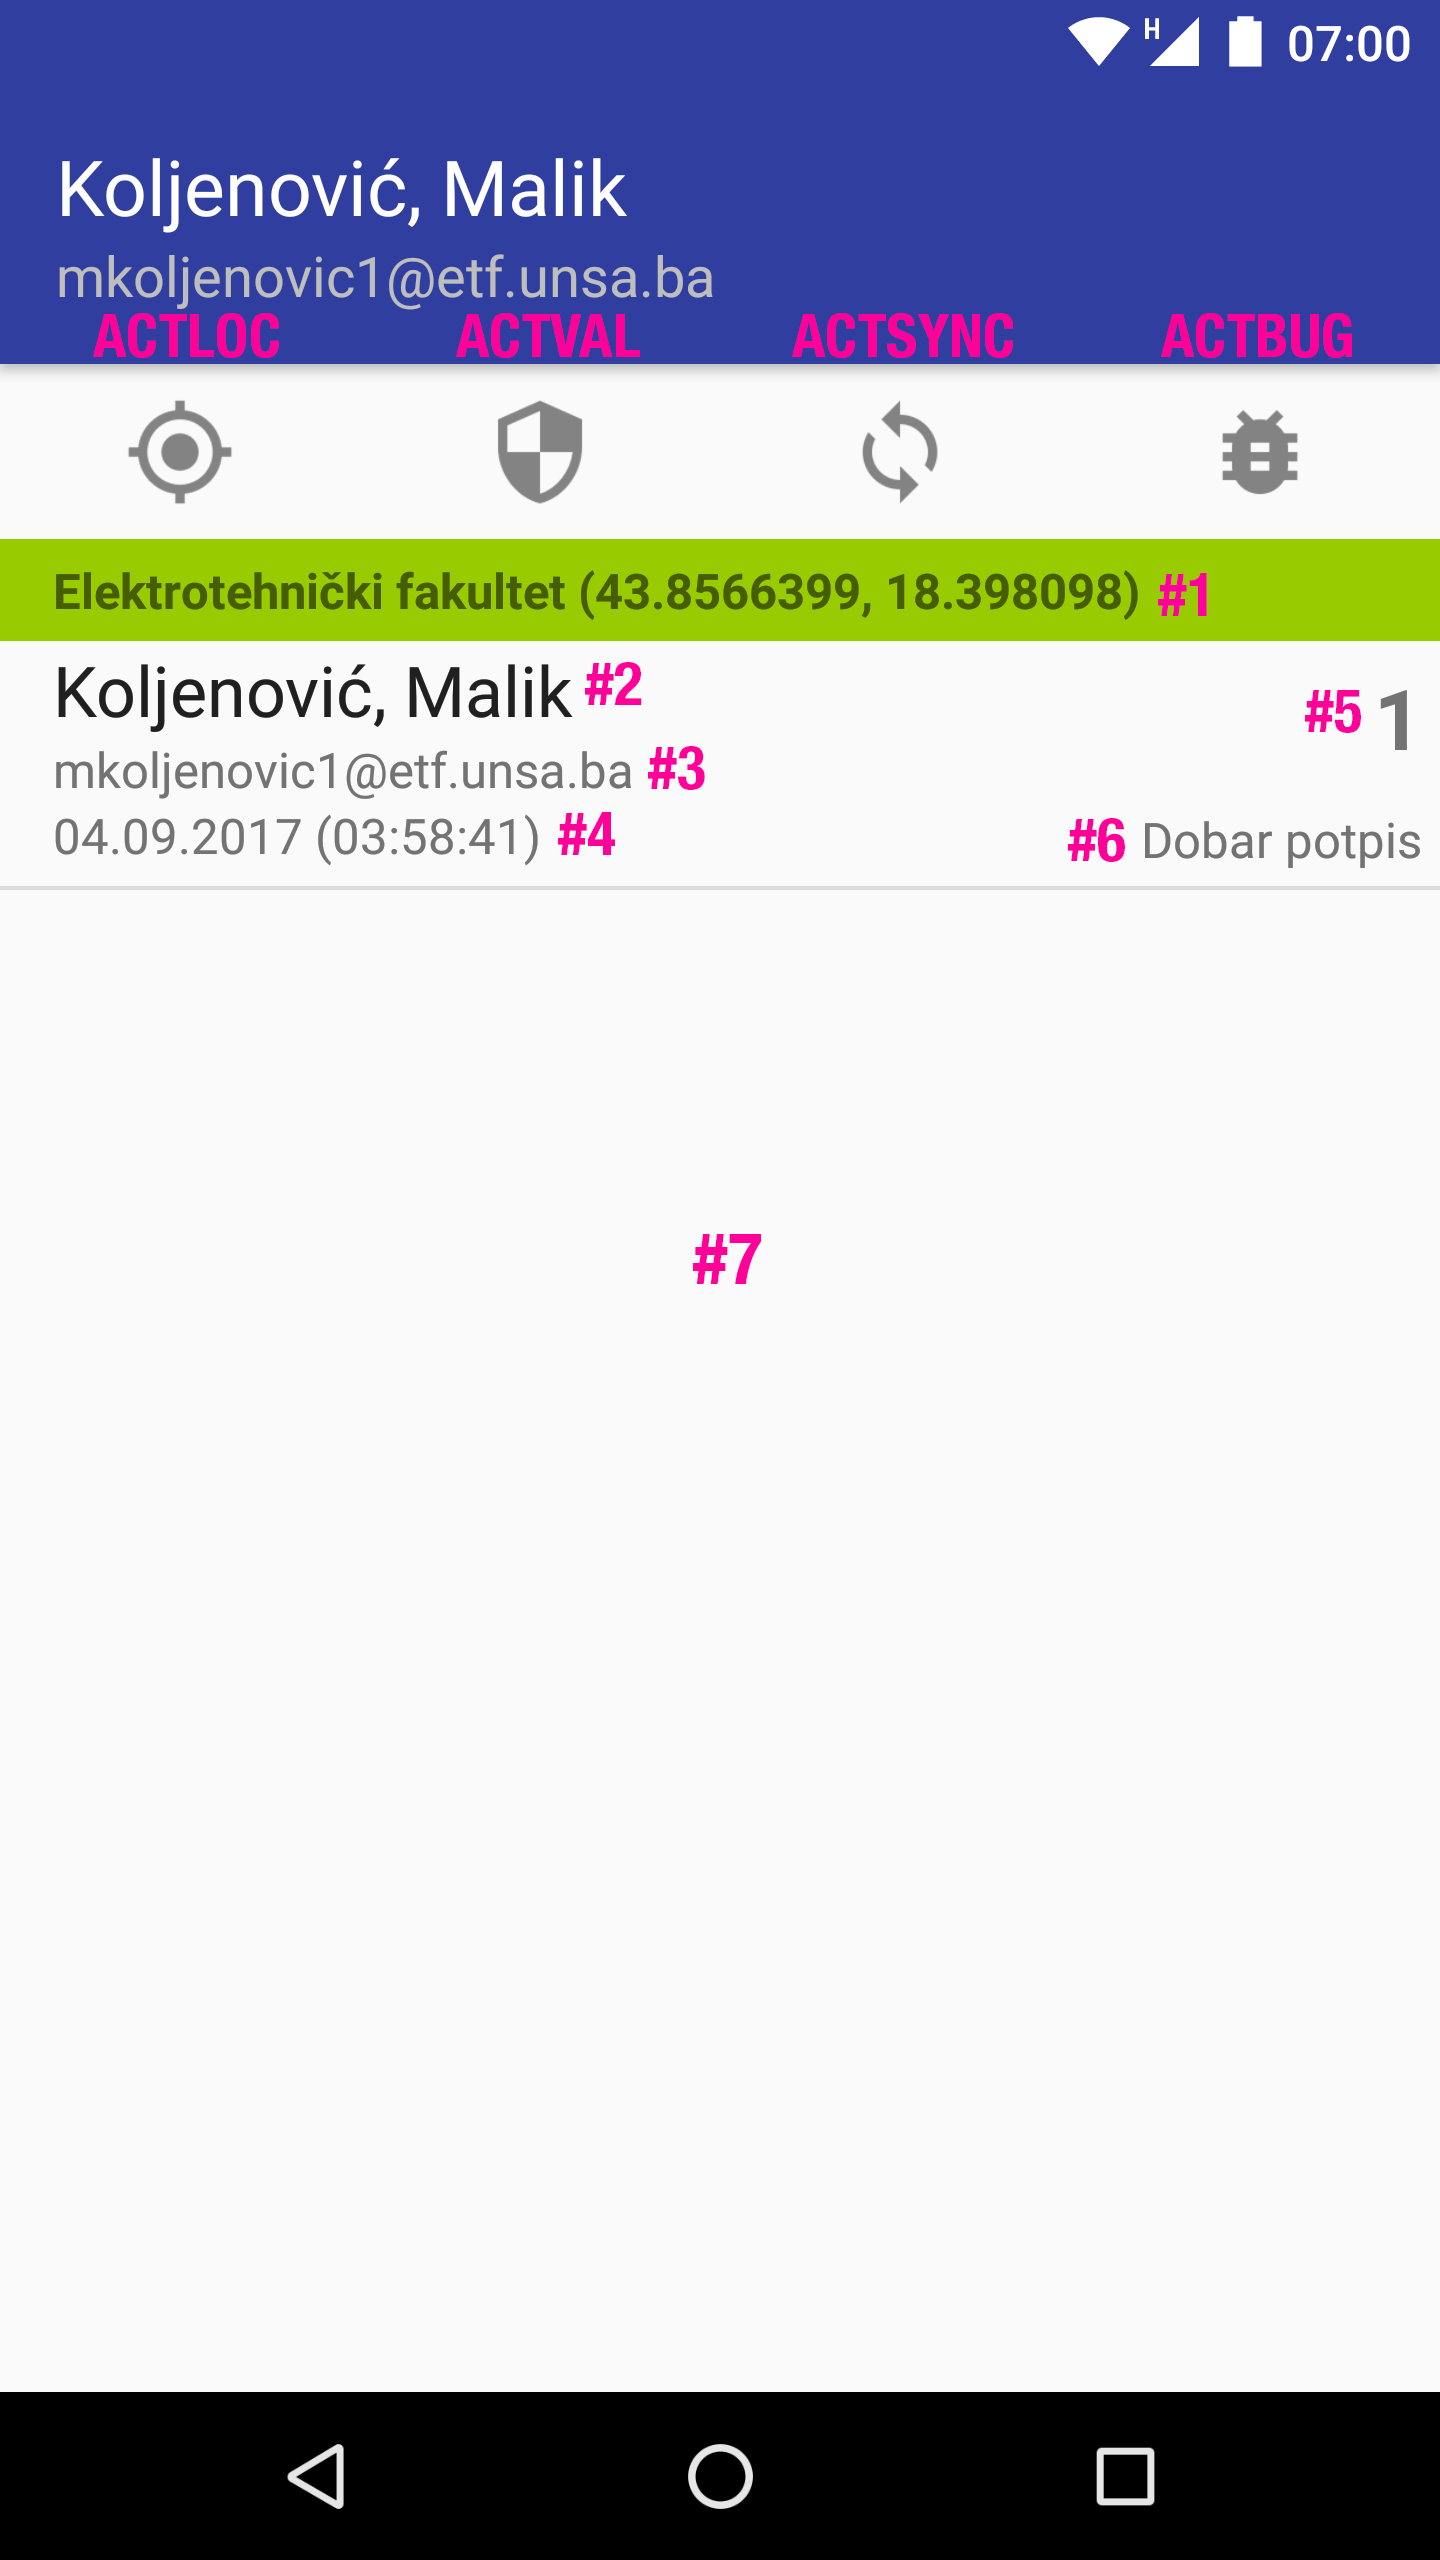
\includegraphics[width=0.9\textwidth]{material/03-verified_annot}
        \caption{UI sesije za prikupljanje potpisa}
        \label{img:ui_r}
    \end{subfigure}
    \caption{Logit UI Android prikaz korisničkog interfejsa}%
    \label{fig:ui}
\end{figure}

\begin{description}[noitemsep,align=right,labelwidth=2cm]
    \item [ACTLOC] služi za ručno osvježavanje trenutne lokacije
    \item [ACTVAL] vrši provjeru valjanosti ključeva prikupljenih pri bilježenju prisustva
    \item [ACTSYNC] sinhronizacija trenutne sesije na LAPI
    \item [ACTBUG] otvara e-mail klijent po izboru korisnika u cilju lakše prijave grešaka
\end{description}

\begin{description}[noitemsep,align=right,labelwidth=2cm]
    \item [\#1] ažurna GPS lokacija uređaja sa nazivom toponima (reverzna geolokacija)
    \item [\#2] ime i prezime jednog korisnika čiji je potpis prikupljen
    \item [\#3] jedinstveni identifikator potpisanog korisnika
    \item [\#4] datum i vrijeme potpisa
    \item [\#5] redni broj potpisa unutar trenutne sesije
    \item [\#6] klikom na ACTVAL korisnik koji prikuplja potpise tokom sesije može od LAPI zatražiti provjeru valjanosti potpisa unutar sesije, povratna informacija prikazana je u ovom polju, ukoliko provjera nije izvršena prostor je prazan
    \item [\#7] po uzoru na potpis sa rednim brojem 1, ovaj prostor sadrži nastavak uzlazno numerisane i silazno sortirane liste prikupljenih potpisa u toku jedne sesije, ACTSYNC nakon uspješne pohrane čisti sve unose iz ove liste
\end{description}

\paragraph*{}
Za korištenje LAPP u NFC emulacijskom modu, kao uređaja za prijavu prisustva - nije potrebno pokretati korisnički interfejs, dovoljno je jednom nakon instalacije izvršiti prijavu i aplikacija će se izvršavati u pozadini, te kada se želi prijaviti prisustvo upaliti ekran studentskog uređaja i prisloniti ga na nastavnički uređaj koji ima pokrenutu UI sesiju za prikupljanje prisustva. Detaljne upute za krajnje korisnike date su u dodatku \ref{ch:man}.